% !TEX root = main.tex
\section{アクチュエータ,センサの動作確認}

\subsection{2軸ロボット実験装置におけるアクチュエータとセンサ}

\begin{figure}[H]
    \centering
    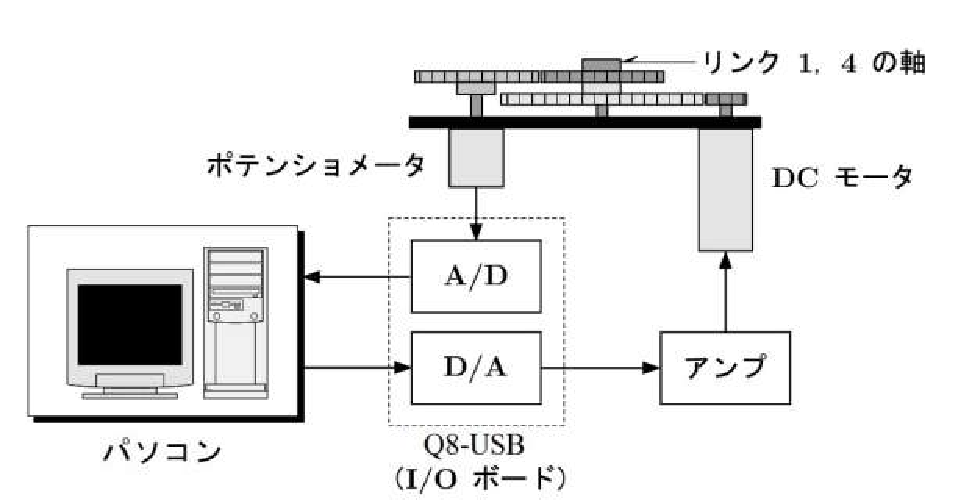
\includegraphics[width=0.8\linewidth]{figure/actuator_sensor.pdf}
    \caption{アクチュエータ(DCモータ)とセンサ(ポテンショメータ)}
    \label{fig:actuator_sensor}
\end{figure}

図\ref{fig:actuator_sensor}に示すように,2軸ロボット実験装置はリンク1,リンク4がギアを介してDCモータにより回転するようになっている.
DCモータを駆動させるためにパソコンにより計算された指令電圧は,I/OボードQ8-USBでD/A変換された後,アンプを介してDCモータに入力される.
また,リンク1,リンク4の回転角は角度センサであるポテンショメータにより電圧値として検出され,I/OボードQ8-USBでA/D変換された後,パソコンに取り込まれている.

\subsection{D/A変換とアクチュエータの動作確認}
\subsubsection{実験装置のセッティングと\textbf{MATLAB}/Simulinkの起動}

図\ref{fig:experiment_setup}に示すように,実験装置の2つの軸にそれぞれリンクを取り付ける.
また,図\ref{fig:terminal_connection}のようにターミナル,Universal Power Module,2軸ロボットのケーブルが接続されていることを確認する.
ただし,左側のDCモータおよびポテンショメータに対するチャネルを\textbf{CH0}(チャネル0),
右側のDCモータおよびポテンショメータに対するチャネルを\textbf{CH1}(チャネル1)とする.


\begin{figure}[H]
    \centering
    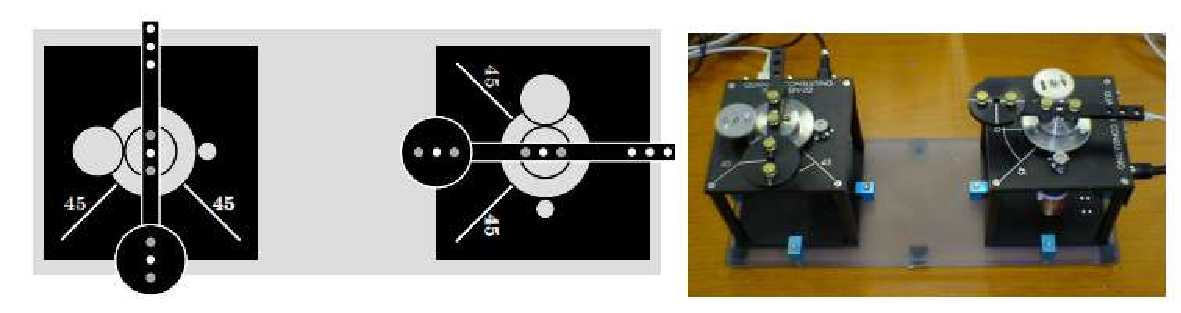
\includegraphics[width=0.8\linewidth]{figure/experiment_setup.pdf}
    \caption{実験装置}
    \label{fig:experiment_setup}
\end{figure}

\begin{figure}[H]
    \centering
    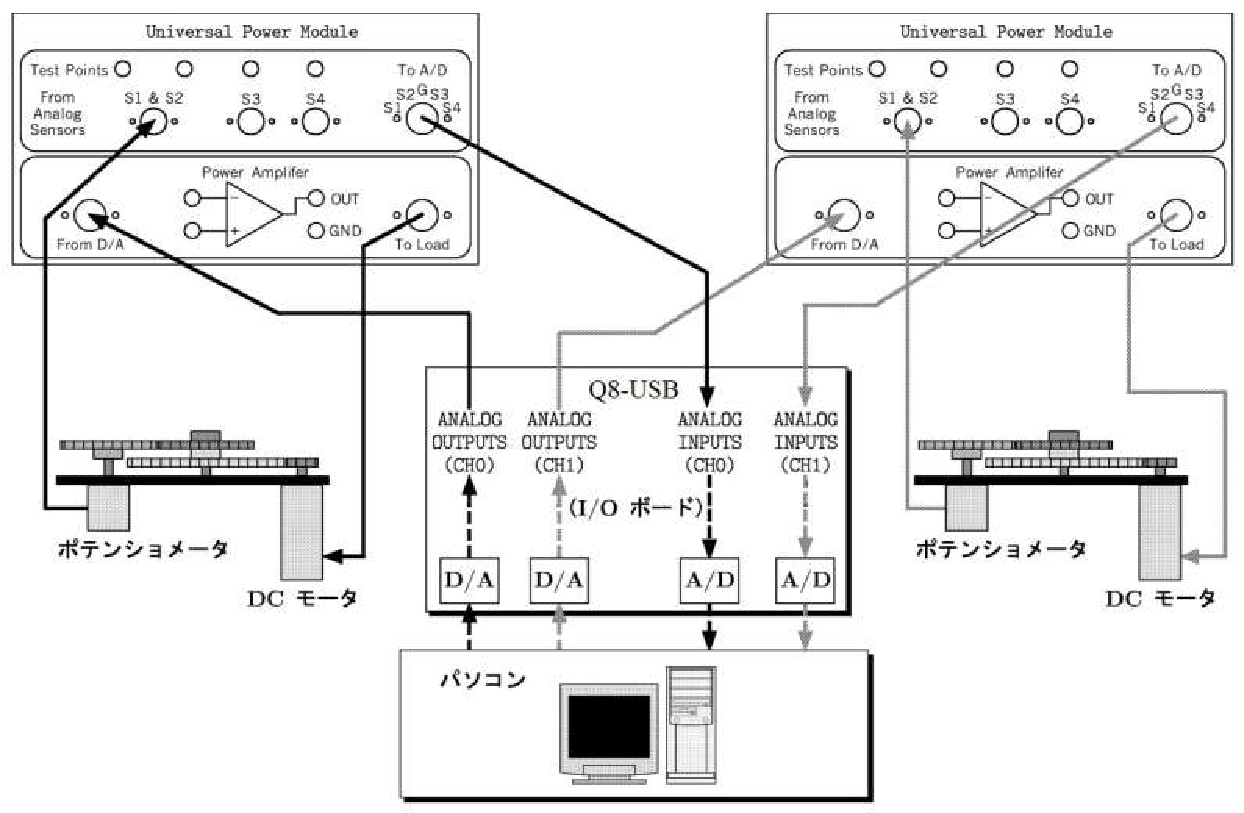
\includegraphics[width=0.95\linewidth]{figure/terminal_connection.pdf}
    \caption{実験装置の接続}
    \label{fig:terminal_connection}
\end{figure}

つぎに,Windowsスタートメニューより MATLAB R2013a を起動する.MATLAB のコマンドウィンドウ上で以下のように入力し,カレントディレクトリ(作業するフォルダ)を変更する.(Xは自分の班名に置き換える.)

\begin{tcolorbox}[colback=white,colframe=black]
    \verb|cd D:\student_senkouka\group_X|
    \end{tcolorbox}

    \subsubsection{モデルの移動と結線}

    左右のDCモータに2\,[V]の電圧を加えたときのリンクの動きを調べてみよう。
    MATLABの“現在のフォルダー”にある,“da”フォルダーを選択し,“da\_conv.slx”をダブルクリックしてSimulinkモデルを起動する。
    起動したモデルを図\ref{fig:da_conv}のように結線する。
    また,各ブロックをダブルクリックして,パラメータを変更する。
    

    \begin{figure}[H]
        \centering
        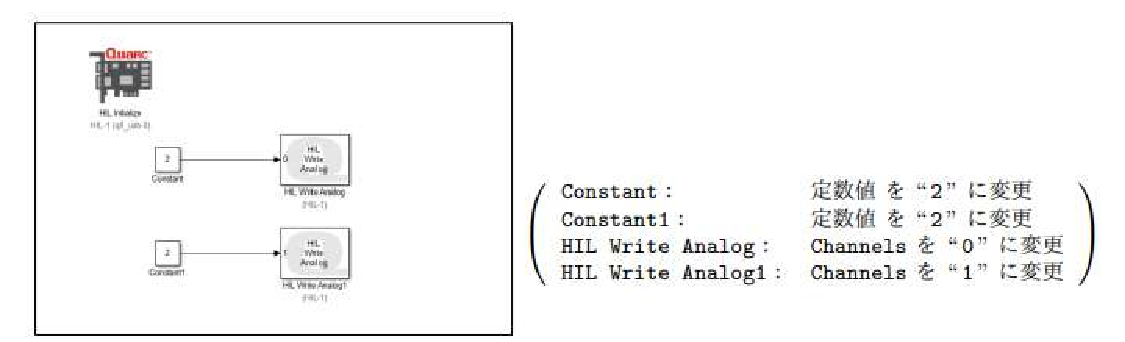
\includegraphics[width=0.8\linewidth]{figure/da_conv.pdf}
        \caption{da\_conv.slx}
        \label{fig:da_conv}
    \end{figure}
    
    \subsubsection{Simulation Parameters のパラメータ設定}

    Simulink モデルウィンドウのツールバーから``モデルコンフィグレーションパラメーター''を選択し,
    ``ソルバー''を選択,図 \ref{fig:sim_param} のようにパラメータを設定する.
    
    \begin{figure}[H]
        \centering
        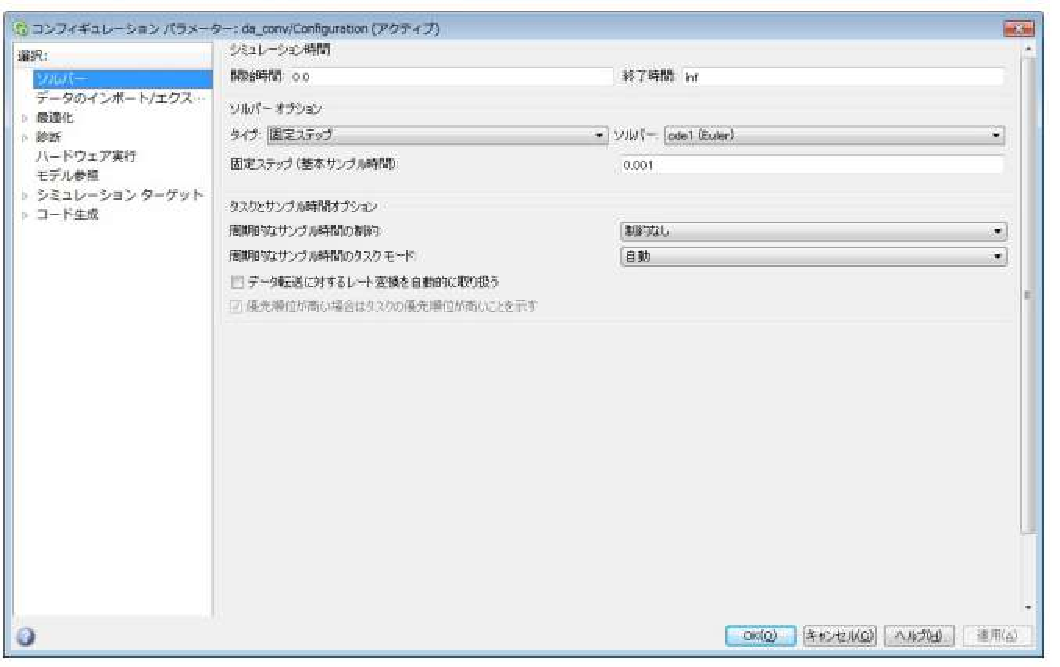
\includegraphics[width=0.8\linewidth]{figure/sim_param.pdf}
        \caption{Simulation Parameters のパラメータ設定}
        \label{fig:sim_param}
    \end{figure}
    
    \subsubsection{コンパイル}
    Dドライブのディレクトリ(フォルダ)D:\textbackslash student\_senkouka\textbackslash group\_X\textbackslash 
    da(Xは自分の班名)がカレントディレクトリとなっているかどうか確かめる.
    カレントディレクトリとなっていない場合は現在のフォルダーを操作してカレントディレクトリを変更する.
    
    \begin{figure}[H]
        \centering
        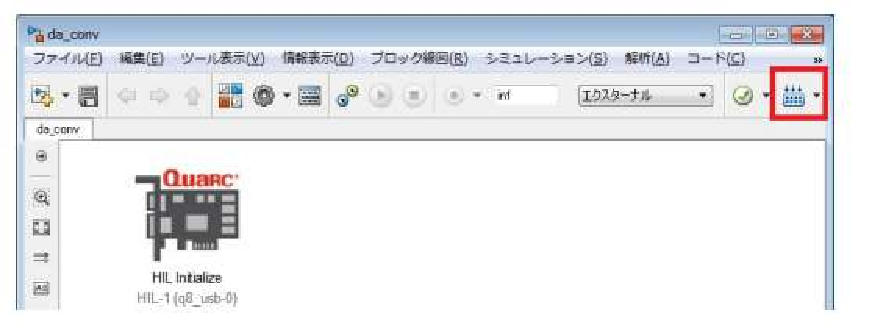
\includegraphics[width=0.8\linewidth]{figure/compile_button.pdf}
        \caption{コンパイル}
        \label{fig:compile_button}
    \end{figure}
    